\documentclass[11pt]{article}

\usepackage{amssymb}
\usepackage{amsmath}
\usepackage{graphicx}
\usepackage{cite}
\usepackage{xparse}
\usepackage[table]{xcolor}
%\usepackage{algorithmic}
%\usepackage{algorithm}
\usepackage{todonotes}
\usepackage{url}
\usetikzlibrary{arrows}
\usepackage{booktabs}
\usepackage{tikz}
\usetikzlibrary{calc,fit,shapes}

\usepackage{caption}
\usepackage{subcaption}


\usepackage{listings}
 \lstset{
            language=Matlab,                                % choose the language of the code
    %       basicstyle=10pt,                                % the size of the fonts that are used for the code
            numbers=left,                                   % where to put the line-numbers
            numberstyle=\footnotesize,                      % the size of the fonts that are used for the line-numbers
            stepnumber=1,                                           % the step between two line-numbers. If it's 1 each line will be numbered
            numbersep=5pt,                                  % how far the line-numbers are from the code
    %       backgroundcolor=\color{white},          % choose the background color. You must add \usepackage{color}
            showspaces=false,                               % show spaces adding particular underscores
            showstringspaces=false,                         % underline spaces within strings
            showtabs=false,                                         % show tabs within strings adding particular underscores
    %       frame=single,                                           % adds a frame around the code
    %       tabsize=2,                                              % sets default tabsize to 2 spaces
    %       captionpos=b,                                           % sets the caption-position to bottom
            breaklines=true,                                        % sets automatic line breaking
            breakatwhitespace=false,                        % sets if automatic breaks should only happen at whitespace
            escapeinside={\%*}{*)}                          % if you want to add a comment within your code
}


\setlength{\paperwidth}{8.5in}
\setlength{\paperheight}{11in}
\setlength{\voffset}{-0.2in}
\setlength{\topmargin}{0in}
\setlength{\headheight}{0in}
\setlength{\headsep}{0in}
\setlength{\footskip}{30pt}
\setlength{\textheight}{9.25in}
\setlength{\hoffset}{0in}
\setlength{\oddsidemargin}{0in}
\setlength{\textwidth}{6.5in}
\setlength{\parindent}{0in}
\setlength{\parskip}{9pt}

\newcommand{\ben}{\begin{enumerate}}
\newcommand{\een}{\end{enumerate}}

\DeclareGraphicsRule{.JPG}{eps}{*}{`jpeg2ps #1}

\title{Project: Streaming Graph Partitioning}
\author{Casey Battaglino\\Robert Pienta}
%\date{}
\begin{document}
\maketitle

\begin{abstract}
Graph partitioning is the process of dividing a graph into subgraphs such that the number of edges between subgraphs is reduced. Our project investigates the process of partitioning a graph using a \emph{streaming} partitioner, which must make partition decisions as each vertex is read from memory, simulating an online algorithm that must process nodes as they arrive. In this project, we demonstrate and analyze streaming graph partitioning on a wide spectrum of real-world and synthetic graphs, as well as explore ways of improving partition quality. 
\end{abstract}

\section{Graph Partitioning} \vspace{-10 pt}
Graph partitioning has been a standard problem in theoretical computer science for decades, but has seen increasing attention since the 1990s as a method of partitioning problems to increase parallel locality. The balanced graph partitioning problem can be stated as such: we wish to partition the nodes of a graph into $k$ components with capacity $(1+\epsilon)\frac{N}{k}$, such that cost is minimized, where cost is generally the number of edges that cross partition boundaries. While satisfying either the capacity constraint or the partitioning objective on their own is trivial, requiring both balance and cost-minimization places this problem in NP-complete, because it becomes a minimum-bisection problem~\cite{Garey:1979:CIG:578533}.

\begin{figure}[ht]
\centering
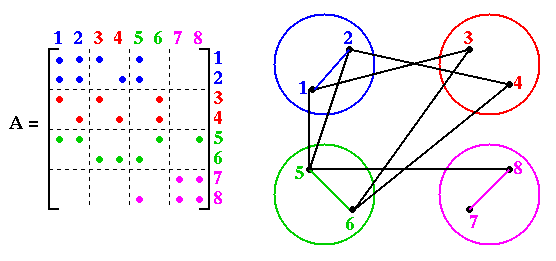
\includegraphics[scale=.60] {figures/graphpart.png}
\caption[Caption for]{Graph 4-partition shown with corresponding adjacency matrix \footnotemark}
\label{fig:0}
\end{figure}

\footnotetext{Source: Jim Demmel's CS267 Lectures,~\url{http://www.cs.berkeley.edu/~demmel/cs267}}

Offline graph partitioning algorithms, where the graph is allowed to exist in memory with total information about edges, have existed for decades. Hundreds of variants of such algorithms likely now exist, and range from spatial methods~\cite{Gilbert95geometricmesh} to spectral methods~\cite{arora2009expander}. The most scalable and effective graph partitioners on massive datasets are currently multi-level partitioners, which recursively contract the graph to a small number of vertices, and then heuristically optimize the problem on each subsequent expansion~\cite{karypis1998multilevel}. 

\section{Streaming Graph Partitioning}\vspace{-10 pt}
Streaming graph partitioning has only been introduced in the last couple of years~\cite{DBLP:journals/corr/abs-1212-1121,Stanton:2012:SGP:2339530.2339722,tsourakakis2012fennel}, as graphs grow to the point where they may not fit into memory, or must be distributed to compute nodes on the fly. In the streaming model, input data (vertices) arrive sequentially from a generating source (such as a web-crawler), and must be partitioned as they arrive. As an example, partitioning a 26GB Twitter follower graph can take nearly a day using the fastest offline algorithms, but can take a matter of minutes using a streaming algorithm.

Streaming partitioning is dependent on the order in which vertices arrive. For instance, a web crawler might generate vertices in an order that represents a Breadth-First or Depth-First traversal of the web, or we may receive vertices in a random order. An analysis of streaming algorithms may also consider an adversarial ordering that produces the worst possible results~\cite{Stanton:2012:SGP:2339530.2339722}. For the purposes of this project we always consider a random ordering. 

\subsection{Streaming Heuristics}
Assuming vertices arrive in some order, a heuristic makes a partition decision, given vertex $v$, and capacity constraint $C$ (where $C$ is generally $\approx \frac{(\epsilon+|V|)}{n}$ Stanton presents the following heuristics, roughly in order from most naive to most complex~\cite{Stanton:2012:SGP:2339530.2339722}: (only the un-buffered heuristics are presented)

\begin{enumerate}
\item \textbf{Balanced:} assign $v$ to partition of minimum size, with random tie breaking.
\item \textbf{Chunking:} divide input stream into chunks of size $C$.
\item \textbf{Hashing:} assign $v$ to $H(v)$, where $H$ is hash function $F:V\to\{1\dots k\}$
\item \textbf{Weighted Deterministic Greedy (WDG):} Assign $v$ to partition that it has most edges to, weighted by the relative size of each partition (weight function can be linear or exponential).
\item \textbf{Weighted Randomized Greedy:} Assign $v$ randomly according to a probability distribution defined by the weights of each partition in WDG.
\item \textbf{Weighted Triangles:} Assign $v$ to partition whose intersection with $v$ contains the most triangles, weighted by the relative size of each partition.
\item \textbf{Balance Big:} for high-degree $v$, use Balanced. For low-degree $v$, use WDG. 
\end{enumerate}

Of note is that many major graph-processing toolkits such as GraphLab~\cite{Low:2012:DGF:2212351.2212354} use the hashed (random) partitioning method, which essentially produces a worst-case edgecut of size $\frac{k-1}{k}|E|$, but which has the benefit that $H(v)$ can be called at any time to return the compute node that owns $v$. 

In Stanton's experimental results~\cite{Stanton:2012:SGP:2339530.2339722}, WDG performed far better than any other partitioner. FENNEL~\cite{tsourakakis2012fennel} is a heuristic that generalizes the WDG partitioner for any weight function, and provides a somewhat more rigorous theoretical framework. 

\subsubsection{FENNEL Heuristic}

\subsection{Possible Advantages of Streaming Partitioning}
The most salient property of streaming partitioning is its speed: it can partition the graph in a single sweep, with $O(|E|)$ memory access, storage, and run time. Existing graph partitioners require the whole graph to be represented in memory, whereas streaming graph partitioning can process vertices as they arrive.

Another qualitative advantage that we propose is the

\section{Implementation}
Our first goal was to implement the generalized WDG partitioner FENNEL, and test it on a wide variety of real-world and synthetic graphs. Our initial `test-bed' was implemented in MATLAB, because many important properties of graphs can be easily extracted using vector notation on their adjacency matrices. As we scaled to larger graphs, the outer for-loop in the code (which iterates over each vertex) began to take an infeasible amount of time, so we implemented a more fully-featured test-bed in C. Our code is located at~\url{https://github.com/cjbattagl/graphpart/}

\subsection{Features}
Our implementation can read graphs in three formats (Harwell-Boeing, Matlab, and Matrix-Market Formats). This allows us to read in the entire SNAP graph archive~\cite{Leskovec-data}. It can read in symmetric (undirected) and unsymmetric (directed) graphs. Once the graph is read in, we convert it from unordered triplet format to Compressed Sparse Row format, which allows us to iterate through the neighbor list of any node in linear time, as well as compute the degree of any node in constant time.

Once we have our graph stored as a matrix in CSR form, we can perform a simulation of streaming $k-$partitioning. First we generate the traversal order of the graph (a random vertex order, which we generate using a Knuth Shuffle). We maintain a data structure that contains the assignment of every assigned vertex to its partition. Thus, for a given vertex, we can compute the number of edges from that vertex to each partition by iterating over each edge incident to the vertex. We also maintain a running total of vertices in each partition. This process lets us compute the FENNEL algorithm in $O(|E|)=O(nnz(A))$ time. 

\subsection{Evaluation}

We measured the overall quality of partitions by the \textit{fraction of cut edges} $\lambda$.
\begin{align}\lambda = \frac{\text{Number of edges cut by partition}}{\text{Total number of edges}}\end{align}

In general, we can compare this to the expected quality of a random partition:
\begin{align}\lambda_r = \frac{k-1}{k} \end{align}

\subsubsection{SNAP Data Set}

\begin{figure}[ht]
\centering
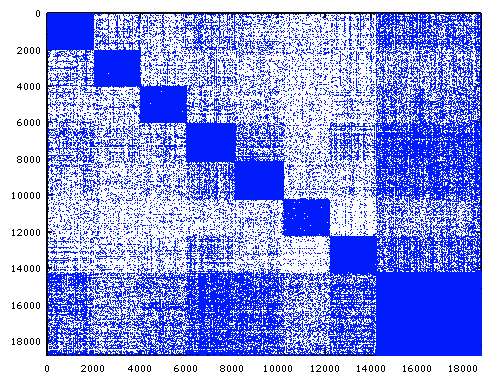
\includegraphics[scale=.70] {figures/astroPh8.png}
\caption[Caption for]{Spy plot of ca-AstroPh 8-partition ($\lambda=0.253$)}
\label{fig:3}
\end{figure}

\begin{figure}[ht]
\centering
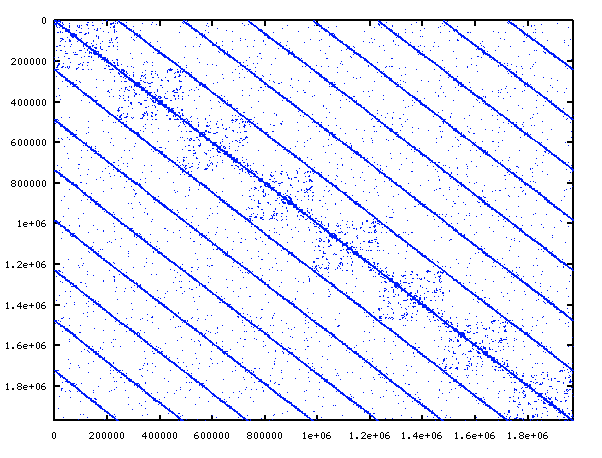
\includegraphics[scale=.60] {figures/roadNet-CA8.png}
\caption[Caption for]{Spy plot of roadNet-CA 8-partition ($\lambda=0.177$). This illustrates how a streaming algorithm cannot take into account the spatial/planar properties of a graph.}
\label{fig:4}
\end{figure}


\begin{figure}
\caption{Basic properties of graphs in SNAP data set with $\lambda$ for one pass}
\rowcolors{2}{green!25}{yellow!30}
\centering
{ \begin{tabular}{ *6l }    \toprule
\emph{Data Set} & $N$ & $nnz$ & \emph{sym} & \emph{power-law?} & $\lambda$ \\\midrule 
amazon0302 & 262111 & 1234877 & no & yes & 0.2\\ 
amazon0312 & 400727 & 3200440 & no & yes & 0.2\\ 
amazon0505 & 410236 & 3356824 & no & yes & 0.2\\ 
amazon0601 & 403394 & 3387388 & no & yes & 0.2\\ 
as-735 & 7716 & 26467 & yes & yes & 0.2\\ 
as-caida & 31379 & 106762 & no & yes & 0.2\\ 
as-Skitter & 1696415 & 22190596 & yes & yes & 0.2\\ 
ca-AstroPh & 18772 & 396160 & yes & yes & 0.2\\ 
ca-CondMat & 23133 & 186936 & yes & yes & 0.2\\ 
ca-GrQc & 5242 & 28980 & yes & yes & 0.2\\ 
ca-HepPh & 12008 & 237010 & yes & yes & 0.2\\ 
ca-HepTh & 9877 & 51971 & yes & yes & 0.2\\ 
cit-HepPh & 34546 & 421578 & no & yes & 0.2\\ 
cit-HepTh & 27770 & 352807 & no & yes & 0.2\\ 
cit-Patents & 3774768 & 16518948 & no & yes & 0.2\\ 
email-Enron & 36692 & 367662 & yes & yes & 0.2\\ 
email-EuAll & 265214 & 420045 & no & yes & 0.2\\ 
Oregon-1 & 11492 & 46818 & yes & yes & 0.2\\ 
Oregon-2 & 11806 & 65460 & no & yes & 0.2\\ 
p2p-Gnutella04 & 10879 & 39994 & no & yes & 0.2\\ 
roadNet-CA & 1971281 & 5533214 & yes & no & 0.2\\ 
roadNet-PA & 1090920 & 3083796 & yes & no & 0.2\\ 
roadNet-TX & 1393383 & 3843320 & yes & no & 0.2\\ 
soc-Epinions1 & 75888 & 508837 & no & yes & 0.2\\ 
soc-LiveJournal1 & 4847571 & 68993773 & no & yes & 0.2\\ 
soc-sign-epinions & 131828 & 841372 & no & yes & 0.2\\ 
soc-sign-Slashdot081106 & 77357 & 516575 & no & yes & 0.2\\ 
soc-Slashdot0811 & 77360 & 905468 & no & yes & 0.2\\ 
soc-Slashdot0902 & 82168 & 948464 & no & yes & 0.2\\ 
web-BerkStan & 685230 & 7600595 & no & yes & 0.2\\ 
web-Google & 916428 & 5105039 & no & yes & 0.2\\ 
web-NotreDame & 325729 & 1497134 & no & yes & 0.2\\ 
web-Stanford & 281903 & 2312497 & no & yes & 0.2\\ 
wiki-Talk & 2394385 & 5021410 & no & yes & 0.2\\ 
wiki-Vote  & 8297 & 103689 & no & yes & 0.2\\ 
 \hline
\end{tabular}\par
}
\end{figure}

\dots

\subsubsection{Synthetic Graphs}
\dots

\section{Additional Passes}
Another operation we explored was performing additional passes of partitioning on a pre-partitioned graph. The reasoning is that the partitioner is fast enough that it may be faster to do $n$ passes than use a slower mainstream graph partitioner, for some value of $n$. To explore this idea, we perform a number of passes on the SNAP data set, and observe qualitatively which graphs benefit the most. 

The algorithm is simple: once we have computed the first partition, we retain the original partition mapping. Then, as we make another pass, we compute the new objective function using the partition mapping that has already been filled in. Vertices may then be switched to new partitions. This mitigates poor partitioning decisions that may have been made at the beginning of the algorithm, when there was not as much information. 

\bibliographystyle{plain}
\bibliography{bib}

\newpage
\appendix
\section{\\Streaming Partitioner Code} \label{App:AppendixA}
% the \\ insures the section title is centered below the phrase: AppendixA

\begin{verbatim}
static int fennel_kernel(int n, int nparts, int *partsize, int *rowptr, int *colidx,
    bool **parts, float alpha, float gamma, int *emptyverts) {
      
  int *partscore = (int*)malloc(nparts * sizeof(int));
  int *row;
  int vert, k, s, nnz_row, best_part, randidx, nededges = 0, node = 0;
  float curr_score, best_score;
  int *vorder = genRandPerm(n);
  int oldpart;

  emptyverts = 0;

  for (int i = 0; i < n; i++) {
    for (s = 0; s < nparts; s++) { partscore[s]=0; }
    vert = vorder[i];
    row = &rowptr[vert];
    nnz_row = *(row+1) - *row;
    oldpart = -1;
   if(nnz_row != 0) {
      // generate partition scores for each partition
      for (k = *row; k < ((*row)+nnz_row); k++) {
        node = colidx[k];
        for (s = 0; s < nparts; s++) { if (parts[s][node]==1) {partscore[s]++;}}
      }
        
      // choose optimal partition (initializing first)
      best_score = (partscore[0]-nnz_row) - calc_dc(alpha,gamma,partsize[0]);
      best_part = 0;
      for (s = 1; s < nparts; s++) {
        curr_score = (partscore[s]-nnz_row) - calc_dc(alpha,gamma,partsize[s]);
        if (curr_score > best_score) { best_score = curr_score; best_part = s; }
      }
      for (s = 0; s < nparts; s++) { 
        if (parts[s][vert] == 1) {
          oldpart = s;
        }
        parts[s][vert] = 0; 
      }
      parts[best_part][vert] = 1;
      partsize[best_part]++;
      if (oldpart >= 0) {
        partsize[oldpart]--;
      }
      
    } else { // empty vertex for some reason... assign it to random permutation
      emptyverts++;
      randidx = irand(nparts);
      for (s = 1; s < nparts; s++) {
        if (parts[s][vert] == 1) {
          oldpart = s;
        }
        parts[s][vert] = 0; 
      }
      parts[randidx][vert] = 1;
      partsize[randidx]++;
      if (oldpart >= 0) {
        partsize[oldpart]--;
      }
    }
  }
  
  free(vorder);
}
\end{verbatim}

\end{document}